\documentclass{article}
\usepackage{fancyhdr,booktabs}
\usepackage{amsmath}
\usepackage{float}
\usepackage{graphicx}
\usepackage{indentfirst}
\usepackage{geometry}
\usepackage{citesort}
\usepackage{titlesec}
\begin{document}


\title{Can We Test Kerr Hypothesis with Extreme-Mass-Ratio Inspirals?}
\author{Xin Shuo\\School of Physics Science and Engineering,\\Tongji University, Shanghai 200092, China}
\date{}
\maketitle
\begin{abstract}
	Future LISA task will be able to detect gravitational waves at $10^{-3}$ to $10^{-1}$ Hz. At this band extreme mass ratio inspiral (EMRI) can be a promising source of signal. In this paper, we investigate possibility of testing Kerr hypothesis against a parametrized non-Kerr metric by matching EMRI signal. However, EMRIs from either equatorial orbits or inclined orbits suffer from the "confusion problem". Our results show that only with very high spin parameter could the small deviation from Kerr be discerned by matching EMRI waveforms.
\end{abstract}


\section{Introduction}

%LIGO 的结果
LIGO's detection of Black Hole (BH) merger event GW150914 has opened the era of Gravitational wave astronomy\cite{ligo}. Observation of  GW170817 \cite{170817}and its electromagnetic counterpart led us to multi-messenger astronomy\cite{multi}. Electromagnetic observation has deepened our understanding of the universe since born of astronomy and the new messenger, gravitational wave, might do even better. With ground-based detectors\cite{a_ligo}\cite{virgo}, space interferometers\cite{lisa_org} and pulsar timing arrays\cite{PTA}, we may observe merger events, EMRI, GW background and etc. These observations that are unaccessible to us previously could potentially deepen our understanding for the universe and fundamental physics.

%LISA
Current ground-based gravitational wave detectors are able to detect gravitational waves (GWs) at relatively high frequency band. Laser Interferometer Space Antenna (LISA), planned to launch in 2030s, will extend the observation band down to milli-Hertz \cite{lisa}. LISA pathfinder has demonstrated desired accuracy by its noise spectrum\cite{LPF} and future LISA task can possibly release enormous scientific yields. By analyzing GW signals at LISA band, we can study the merger history of BHs\cite{lisa_mergerhistory}, probe stellar dynamics\cite{sameOmg} and test gravity theories\cite{test_GR}.

%EMRI
Extreme Mass Ratio Inspiral (EMRI), e.g. a stellar mass compact object (1-10 $M_{\odot}$) orbiting around a Supermassive Black Hole (SMBH), is a promising source of GW signal at LISA band. %EMRI重要性
Although a relatively accurate method to generate waveforms, Teukolsky-based method \cite{TB}\cite{review_waveform}, is computationally expansive, some further approximations, i.e. Numerical Kludge\cite{kludge}, Analytic Kludge\cite{AK} and etc, made the calculation feasible. The analysis of EMRI signal is also sophisticated. Due to low signal-to-noise ratio (SNR), matched filtering has to be utilized in the analysis, and both generating waveform template and matching signal require enormous computation power. Markov-Chain Monte Carlo (MCMC) and Machine Learning might shed some light on it \cite{MCMC} \cite{machine_learning}.

%Testing Kerr metric
One scientific goal of LISA task is testing General Relativity (GR) and Kerr metric around BH. There are already several previous works demonstrating possible constraints LISA can set for alternative metric or theory of gravity. \cite{test_scalar-tensor} shows the bound of coupling constant $\omega$ in scalar-tensor theory that LISA can set. \cite{test_bumpyBH} gives the estimation of the parameter limits for ``Bumpy BH metric'' constrained by EMRI detection. Most works are using the error estimated by Fisher Matrix calculation as the constraint on the parameters. 

%Confusion
However, as \cite{07conf} mentioned, due to large parameter space EMRI has, "confusion problem" can prevent us from parameter estimation and, therefore, testing alternative theory or metric. Namely, two EMRI waveform with different parameters can be almost identical (overlap, as defined in \ref{p_mf}, over 0.97). This problem is demonstrated in \cite{majorPRD} for a special case, i.e. consider an approximate metric describing BH+torus and Kerr metric, confusion problem exists for EMRI emission from equatorial orbits. We try to extend the analysis to continuously parametrized metric and inclined eccentric orbits.

%KRZ parametrization
In order to test No-Hair Theorem, i.e. astrophysical BHs are described only by mass and spin, many model-independent parametrization of BH metric have been proposed. The JP metric proposed by Tim Johannsen and Dimitrios Psaltis\cite{johannsen} and the Johannsen metric proposed by Tim Johannsen \cite{johannsen_final}, both expanding the metric component in power series of $\frac{M}{r}$, are widely used in testing Kerr hypothesis. However, as mentioned in \cite{johannsen_diff}, Johannsen metric has some convergence deficiencies. Such problem can be solved by the parametrization proposed in \cite {KRZ}, expanding the metric functions in power series of $\cos \theta$. Here we use the finite number of deformation parameters as chosen in \cite{cosimoKRZ}, another test of Kerr metric.

%in this paper...
The rest of this paper is organized as follows. In Sec. \ref{p_krz}, general parametrization for BH spacetime is discussed. Sec. \ref{p_wave} introduced the "Kludge" waveform generation method and matched filtering protocol that we used. Then we give our major results about the "confusion" problem for equatorial orbits and inclined orbits in Sec. \ref{p_conf}. Finally, we summarize and discuss the results in Sec. \ref{p_fin}. 

\section{General Parametrization of Metric around Black Hole}
\label{p_krz}


In order to test Kerr hypothesis or General Relativity in a model independent manner, one usually turn to general parametrization of metric describing astrophysical BHs. Instead of using a metric derived from a specific theory, a general metric could enable model-independent test of Kerr hypothesis. One reasonable choice is expand the metric functions in power series of $\frac 1 {r^2+a^2cos^2\theta}$, as adopted by Johannsen and Psaltis. \cite{johannsen}. Under Boyer-Lindquist coordinate, the metric, which we refer to as JP metric, reads:
\begin{equation}
\begin{aligned}
	ds^2=&-[1+h(r,\theta)](1-\frac{2Mr}{\Sigma}) dt^2 - \frac{4aMrsin^2\theta}{\Sigma} [1+h(r,\theta)] dtd\phi + \frac{\Sigma[1+ h(r,\theta) ] }{ \Delta + a^2 \sin^2 \theta h(r,\theta )} dr^2  \\
	&+\Sigma d\theta^2 +[ \sin^2\theta (r^2+a^2 + \frac{2a^2Mr\sin^2\theta }{\Sigma}) + h(r,\theta ) \frac{a^2 (\Sigma +2Mr)\sin^4\theta  }{\Sigma} ] d\phi^2
\end{aligned}
\end{equation}
where
\begin{equation}
	\Sigma=r^2 +a^2\cos^2\theta,\,\,\,\Delta= r^2 - 2Mr +a^2 ,\,\,\,  h(r,\theta ) = \sum_{k=0}^{\infty} (\epsilon_{2k} + \epsilon_{2k+1} \frac{Mr}{\Sigma}) (\frac{M^2}{\Sigma})^k
\end{equation}
%介绍Johannsen metric

When testing Kerr metric, one usually hope the alternative metric still preserve the symmetries of Kerr metric, which are related to three constants of motion. The general form of metric that has three constants of motion is proposed by Johannsen\cite{johannsen_final}. The line element of this parametrization in Boyer-Lindquist coordinates, which we refer to as Johannsen metric, is:
\begin{equation}
\begin{aligned}
	ds^2 =& -\frac{\tilde{\Sigma} [\Delta - a^2 A_2(r)^2 \sin^2\theta ] }{ [ (r^2+a^2)A_1(r) - a^2 A_2(r) \sin^2\theta ]^2 } dt^2 -  \frac{a [(r^2 + a^2 )A_1(r)A_2(r) - \Delta ] \tilde{\Sigma} \sin^2\theta }{ [(r^2+a^2 ) A_1(r) -a^2 A_2(r) \sin^2 \theta ]^2 } dtd\phi\\
	& + \frac{\tilde{\Sigma} \sin^2\theta [(r^2+a^2)^2 A_1(r)^2 - a^2\Delta \sin^2\theta  ]}{ [(r^2+a^2)A_1(r) - a^2 A_2(r) \sin^2 \theta ]^2 } d\phi^2 +\frac{\tilde{\Sigma}}{\Delta A_5(r)} dr^2  + \tilde{\Sigma} d\theta^2
\end{aligned}
\end{equation}

where $\Delta$ is defined in the same way as JP metric, and the functions $A_i(r),\,i=1,2,5$ and $\tilde{\Sigma}$ are expanded in power series of $\frac{M}{r}$

\begin{equation}
\begin{aligned}
	A_i(r) =& 1+ \sum_{n=2}^{\infty} \alpha_{in} (\frac M r)^n\\
	\tilde{\Sigma} =& \Sigma +f(r)\\
	f(r)=&\sum_{n=3}^{\infty} \epsilon_n \frac{M^n}{r^{n-2}}
\end{aligned}
\end{equation}

%Johannsen metric 的问题
Johannsen metric and JP metric have been adopted by several works on testing Kerr metric, which utilize Ironline\cite{t1_Iron} \cite{t4_Iron}, X-ray polarization\cite{t2_XrayPol}, Black Hole shadows\cite{t3_BHShadow} and etc. However, as mentioned in \cite{johannsen_diff} and \cite {KRZ}, Johannsen metric has several deficiencies. One major problem is expanding the function in power series of $1/r$, so that all element in the series are almost equally important near horizon, which puts a burden when testing Kerr hypothesis in strong field regime. As we will discuss in Sec. \ref{p_conf}, we have to study the dynamics as close to the horizon as possible to mitigate the ``confusion''. This convergence problem can be solved by expanding the metric function in power series of $\cos \theta$, as adopted in \cite{KRZ}. The line element around an axisymmetric black hole proposed by Konoplya, Rezzolla and Zhidenko, which we refer to as KRZ metric, is \cite{KRZ}:
\begin{equation}
\begin{aligned}
	ds^2=-\frac{N^2(r,\theta)-W^2(r,\theta)\sin^2\theta}{K^2(r,\theta)} dt^2-2W(r,\theta)r\sin^2\theta dtd\phi \\+ K^2(r,\theta) r^2\sin^2\theta d\phi^2  +\Sigma(r,\theta)(\frac{B^2(r,\theta)}{r^2 N^2(r,\theta)} dr^2+d\theta^2)
\end{aligned}
\end{equation}
Where $\Sigma$ is defined the same as JP metric and the functions $K(r,\theta),\, N(r,\theta),\, W(r,\theta),\, B(r,\theta),\ $ can be expanded by power series of $\cos\theta$. Here we use the same deformation parameter as \cite{cosimoKRZ}, namely $\delta_i, \, i=1,2,3,4,5,6,7,8$ related to the metric functions by

\begin{equation}
\begin{aligned}
N^2&=(1-r_0/r)[ 1-\epsilon_0r_0/r +(k_{00}-\epsilon_0)r_0^2/r^2 +\delta_1 r_0^3/r^3 ] \\
&+ \{ a_{20} r_0^3/r^3 +a_{21} r_0^4/r^4 + k_{21}r_0^3/r^3[ 1+\frac{k_{22}(1-r_0/r) }{1+k_{23}(1-r_0/r)} ]^{-1}   \} \cos^2\theta   \\
B&=1+\delta_4r_0^2 /r^2 +\delta_5r_0^2 \cos^2\theta /r^2\\
W&=[w_{00}r_0^2 /r^2 +\delta_2 r_0^3/r^3 +\delta_3 r_0^3/r^3 \cos^2\theta ]/\Sigma\\
K^2&= 1+aW/r+\{k_{00}r_0^2/r^2 +k_{21}r_0^3/r^3 [ 1+\frac{k_{22}(1-r_0/r) }{1+k_{23}(1-r_0/r)} ]^{-1} \cos^2\theta \}/\Sigma\\
r_0&=1+\sqrt{1-a^2},\,\,\, a_{20}=2a^2/r_0^3,\,\,\, a_{21}=-a^4/r_0^4 +\delta_6 ,\,\,\, \epsilon_0=(2-r_0)/r_0,\,\,\, k_{00}=a^2/r_0^2,\\
 k_{21}&=a^4/r_0^4 -2a^2/r_0^3-\delta_6,\,\,\, w_{00}=2a/r_0^2,\,\,\, k_{22}=-a^2/r_0^2 +\delta_7,\,\,\,  k_{23} = a^2/r_0^2 +\delta_8
\end{aligned}
\end{equation}

Note that here the coordinate $r$ and BH spin $a$ are redefined by $r/M$ and $a/M$ for brevity in the expression. KRZ parametrization only preserves stationarity and axisymmetry. When each $\delta_i$ is set to 0, the metric recovers Kerr metric. In this paper we mainly consider influence of $\delta_1, \, \delta_2$.

%KRZ metric算四极矩,画d1对horizon的影响

\section{Kludge Waveform and Signal Analysis}
\label{p_wave}

In this section we review the Kludge waveform generation method and signal analysis approach. 
%In \ref{p_kludge} the procedure for generating EMRI waveforms is discussed in detail and \ref{p_mf} outlines the definition of inner product and overlap between two signal.


We use the method established in \cite{kludge}, i.e. Kludge waveform, to calculate EMRI signals. The procedure is: regarding the stellar mass object as a point particle, first calculate the trajectory of the particle in a given metric by integrating geodesic equations; then use quadruple formula to get the gravitational wave from geodesics.

In our instance, to calculate the geodesics, we use:
\begin{equation}
	\dot{u^\mu}=-\Gamma^\mu_{\rho\sigma}u^\rho u^\sigma
\end{equation}
\begin{equation}
	\dot{x^\mu}=u^\mu 
\end{equation}
where $x^\mu$ is the Boyer-Lindquist coordinate of the particle, $u^\mu$ is the 4-velocity and $\Gamma^\mu_{\rho\sigma}$ is Christoffel connection. We didn't use conservation of particle mass, energy and angular momentum to reduce equation but to monitor numerical error. Namely at each step of integration, we check the conservation quantities, namely the modulus of 4-velocity, energy $E$ and $z$ component of angular momentum $L_z$ defined by:
\begin{equation}
	-1 = g_{\mu\nu} u^\mu u^\nu
\end{equation}
\begin{equation}
	E = -u_t = - g_{tt} u^t -g_{t\phi} u^\phi
\end{equation}
\begin{equation}
	L_z = u_\phi = g_{t\phi } u^t + g_{\phi\phi} u^\phi
\end{equation}
 and in Kerr cases, we also check Carter constant
 \begin{equation}
 	Q = (g_{\theta\theta} u^\theta)^2 + \cos ^2 \theta (a^2 (\eta^2-E^2) + (\frac{L_z}{\sin \theta})^2 )
 \end{equation}
During the calculation, we keep the relative drift of conserved quantities less than $10^{-7}$.

For stable bounded geodesics, three parameters, i.e. eccentricity $e$, semi-latus $p$ and inclination angle $\iota$, can be used to characterize the orbit. They are defined as:
\begin{equation}
\begin{aligned}
e=\frac{r_a-r_p}{r_a+r_p},\,\,\, p=\frac{2r_a r_p}{r_a+r_p},\,\,\, \iota=\frac \pi 2 -\theta_{min}
\end{aligned}
\end{equation} 
where $r_a$ is apastron, $r_p$ is periastron and $\theta_{min}$ is the minimum of $\theta$ coordinate. In Kerr spacetime, we can determine the three orbit parameters $e,p,\iota$ from three conserved quantities $E,L_z,Q$ and vice versa. In KRZ non-Kerr spacetime, for equatorial orbits, we can still determine $e,p$ by $E,L_z$.

Transform $(r,\,\theta,\,\phi)$ into $(x,\,y,\,z)$ with the definition of spherical coordinate (rather than the Boyer-Lindquist coordinate), namely $x=r\sin\theta \cos \phi,\, y=r\sin\theta\sin\phi,\, z=r\cos\theta$. Then use quadruple formula, i.e.
\begin{equation}
	\bar{h}^{jk}(t,{\rm {x}})= \frac 2 r [\ddot{T}^{jk} (t')]_{t'=t-r}
\end{equation}
\begin{equation}
	I^{jk}=\mu x'^j_p x'^k_p
\end{equation}
where $\bar{h}^{\mu\nu} = h^{\mu\nu} - \frac 1 2 \eta^{\mu\nu} \eta^{\rho\sigma} h_{\rho\sigma} $ is the metric perturbation under trace-reversed gauge

transform the waveform into transverse-traceless gauge (see formula (17) and (23) in \cite{kludge}), and we get the plus and cross component of the waveform observed at latitudinal angle $\Theta $ and azimuthal angle $\Phi$:
\begin{equation}
\begin{aligned}
h_+ =& h^{\Theta\Theta} - h^{\Phi\Phi}\\
=& \{ \cos^2 \Theta [ h^{xx} \cos^2 \Phi + h^{xy} \sin 2\Phi h^{yy} \sin^2 \Phi ] + h^{zz} \sin^2\Theta - \sin 2\Theta [h^{xz} \cos \Phi + h^{yz} \cos \Phi ] \}\\
&- [ h^{xx} \sin^2\Phi - h^{xy} \sin 2\Phi + h^{yy} \cos^2 \Phi ]
\end{aligned}
\end{equation}\\
\begin{equation}
\begin{aligned}
h_\times =& 2 h^{\Theta\Phi} \\
=& 2 \{ \cos\Theta[-\frac 12 h^{xx} \sin 2\Phi + h^{xy} \cos 2\Phi + \frac 12 h^{yy} \sin 2\Phi ] + \sin \Theta [h^{xz} \sin \Phi - h^{yz} \cos \Phi ] \}
\end{aligned}
\end{equation}
With the resulted "plus" and "cross" components, we define our waveform as $h = h_+ + i h_\times$


Matched filtering is the standard technique to be used in LISA analysis. Here we mainly adopt the fitting factor as  a measure of similarity between two waveforms within LISA band. 

The inner product between two signals, $a(t)$ and $b(t)$, is defined by their cross correlation: \cite{product}
\begin{equation}
	(a|b)=4\Re\int \frac{\tilde{a}^*(f) \tilde{b}(f)}{S_n(f)}df =2\int \frac{\tilde{a}^*(f) \tilde{b}(f) +\tilde{a}(f) \tilde{b}^*(f) }{S_n(f)}df
\end{equation}
where $S_n(f)$ is the power spectral density of LISA noise. In our calculation, the analytic fit to the noise spectrum same as \cite{kludge} is used.

The overlap (fitting factor) between two signals is defined as:
\begin{equation}
	\rm {FF}(a,b)=\frac{(a|b)}{\sqrt{(a|a)(b|b)}}
\end{equation}
If the overlap between two waveforms is above 0.97, we regard them as indistinguishable by LISA.

\section{Numerical Results and Analysis}
\label{p_conf}
When we try to identify EMRI signals, the confusion problem, as described in \cite{sameOmg}, could prevent us from discern non-Kerr signal and Kerr signal. Namely an overlap over 0.97 might happen between non-Kerr signals and Kerr ones with certain parameters. In \ref{p_2d} and \ref{p_3d} we show the confusion problem when matching EMRIs from equatorial and inclined orbit 
\subsection{Equatorial orbit}
\label{p_2d}
Given a waveform under spacetime with non-zero deformation parameter, in order to see if there is "confusion problem", we need to decide which waveform under Kerr spacetime is most similar to it and look at their overlap. Here we search for existence confusion problem with similar method as \cite{majorPRD}, i.e. looking at waveforms with same orbital frequency. The orbital frequencies in Kerr spacetime are given in \cite{tauOmg}. In equatorial orbits, there are two frequencies $\omega_\phi$ and $\omega_r$ related to motion of $\phi$ and $r$ coordinates.

\begin{figure}[!ht]
	\centering
	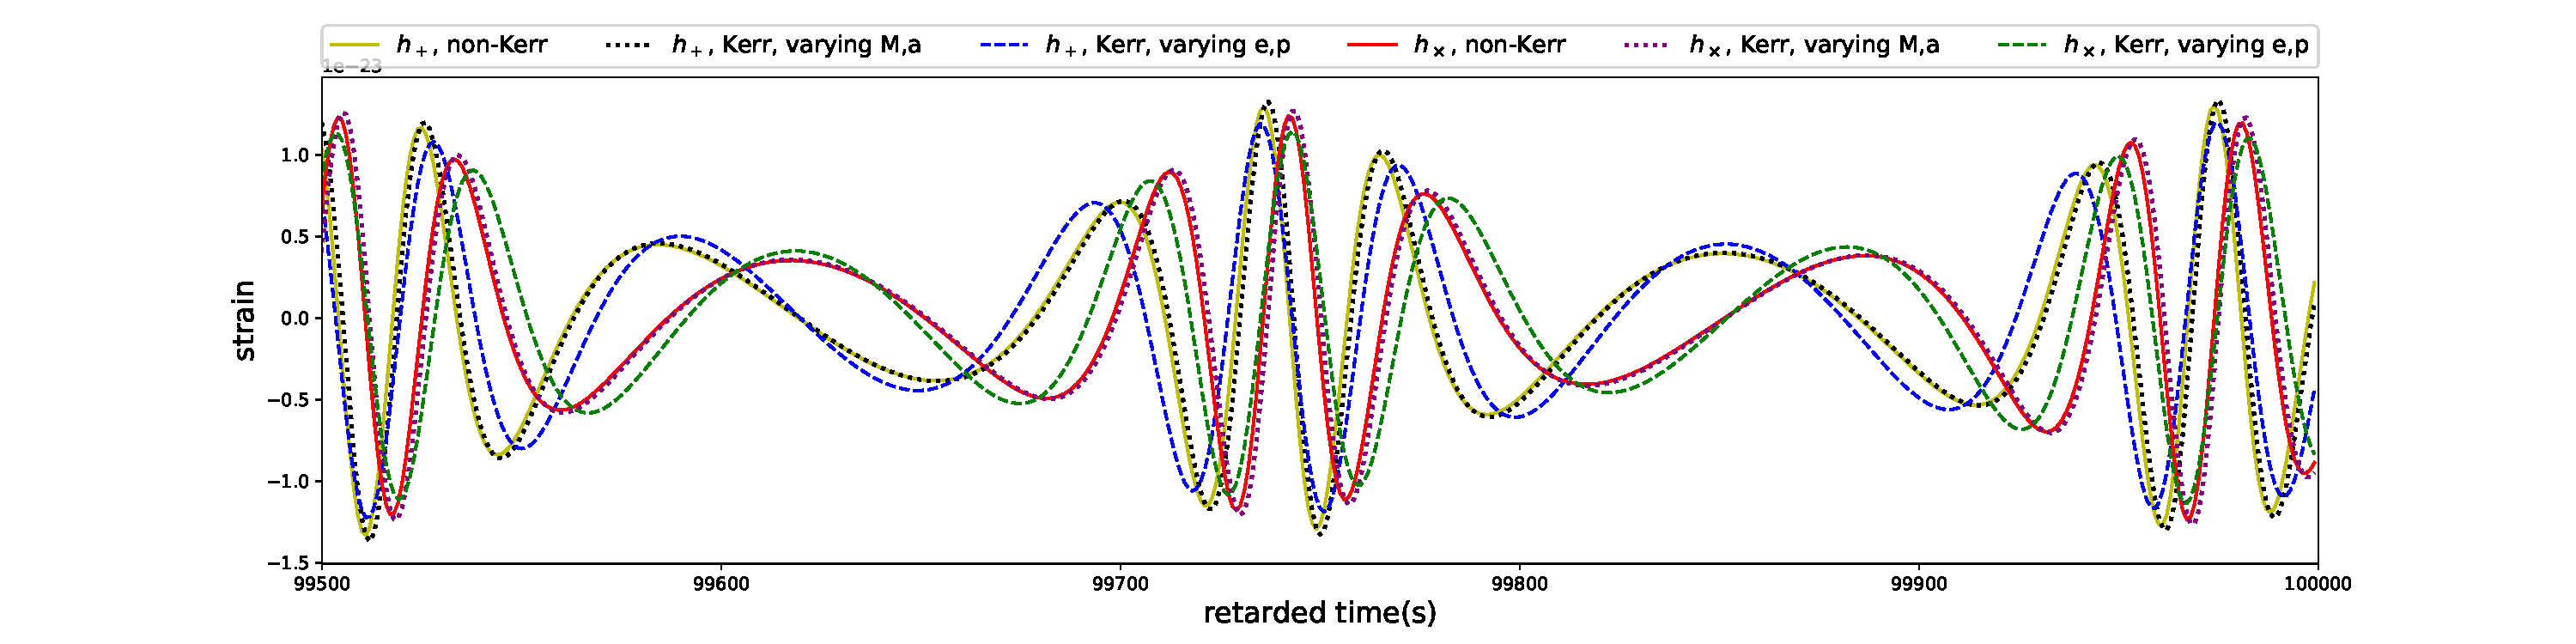
\includegraphics[width=16cm]{eg.pdf}
	
	\caption{"Plus" and "cross" component of EMRIs under non-Kerr spacetime and Kerr spacetime varying $(M,a)$ or $(e,p)$ to equate orbital frequency. The non-Kerr waveform is $(\delta_1,a,M,e,p)=(0,2,0.5,2\times10^5, 0.5,6.0)$. The yellow and red solid lines are "plus" and "cross" component of the non-Kerr waveform. The black and violet dotted lines are "plus" and "cross" component of Kerr waveform with same orbital frequencies as non-Kerr orbit by varying $(M,a)$. The blue and green dashed lines are "plus" and "cross" component of Kerr waveform with same orbital frequencies as non-Kerr orbit by varying $(e,p)$.}
	\label{kkwave}
\end{figure}	

If we restrict ourselves to equatorial motion, set the initial $t$ and $\phi$ to 0 in view of stationarity and axisymmetry and set initial $r=r_{max}$, then the orbit is uniquely determined by orbital eccentricity $e$, semilatus rectum $p$, deformation parameters $\delta_i$, BH mass $M$ and BH spin $a$. As described in \cite{majorPRD}, we can achieve same orbital frequency as non-Kerr signal by varying orbital parameters $e, \,p$ or BH parameters $M, \, a$. So we need to consider EMRIs determined by $(\delta,\, a,\, M,\, e,\, p)$, $(0,\, a,\, M,\, e_{\rm{Kerr}},\, p_{\rm{Kerr}})$ and $(0,\, a_{\rm{Kerr}},\, M_{\rm{Kerr}},\, e,\, p)$. Comparison of waveforms of same orbital frequency is show in Fig. \ref{kkwave}. The overlap between waveforms varying BH mass and spin is over 0.99. In fact, the geodesics that generate the two waves are overlapping.  

\begin{figure}[htb]
	\centering
	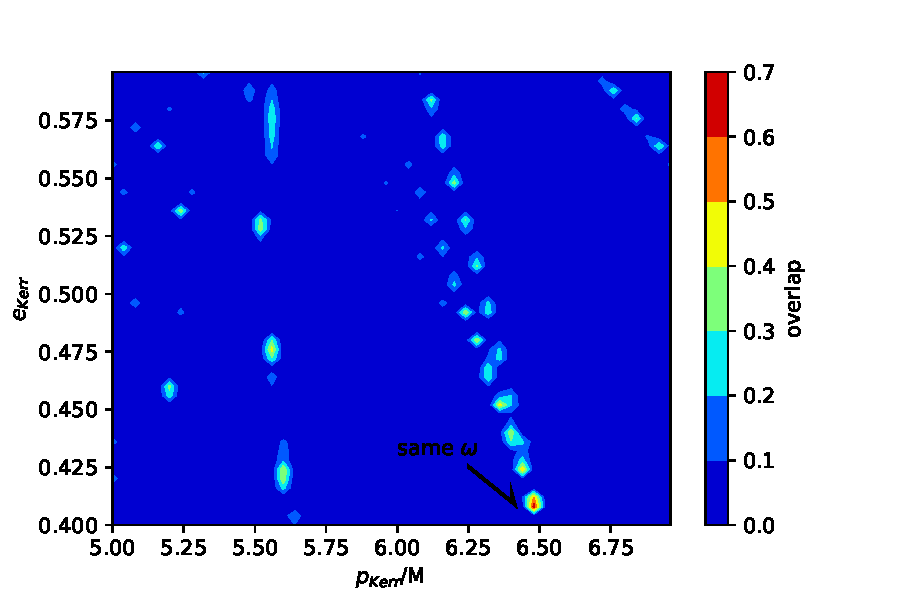
\includegraphics[width=7cm]{OLdist.pdf}
	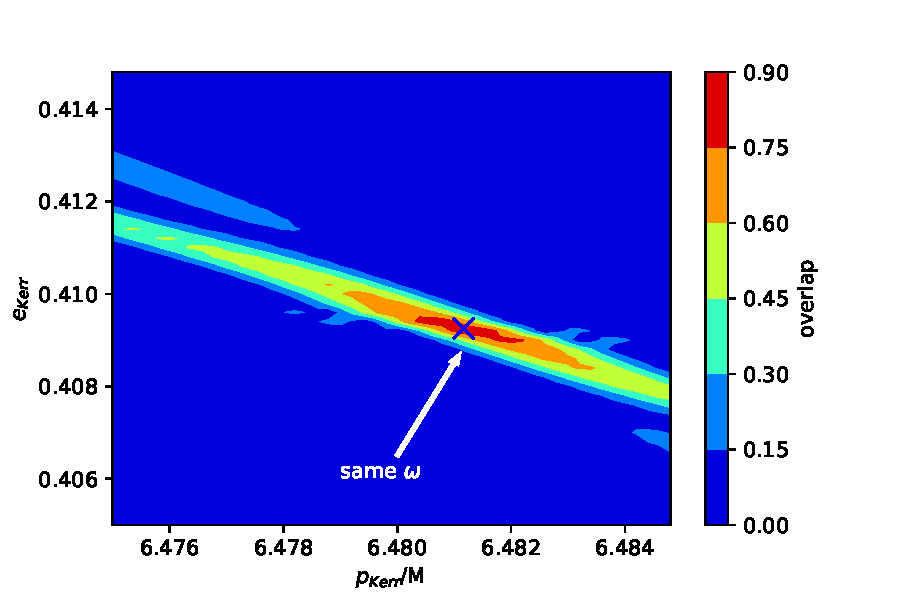
\includegraphics[width=7cm]{OLdist2.pdf}
	
	\caption{Distribution of overlap between waveform of ($\delta_1,\, a,\, M,\, e,\, p$) = (0.2, 0.5, $2 \times 10^5 $, 0.5, 6) and waveforms of ($\delta_1,\, a,\, M,\, e,\, p$) =(0, 0.5, $2 \times 10^5 $, $e_{\rm{Kerr}}$, $p_{\rm{Kerr}}$) on ($e_{\rm{Kerr}}$, $p_{\rm{Kerr}}$) plane. blue cross mark pointed by the arrow: same $\omega_r$ and $\omega_\phi$ at ($e_{\rm{Kerr}}$, $p_{\rm{Kerr}}$) = (0.409248, 6.481170).  The grid size is 50*50.}
	\label{overlapdist}
\end{figure}

According to Ref. \cite{sameOmg}, orbits with same orbital frequency $\omega_r$ and $\omega_\phi$ can generate gravitational waveforms potentially confused with non-Kerr signals. Therefore the overlap between a non-Kerr waveform and several Kerr waveforms should have a local maximum around the parameter leading to same orbital frequency. Here we check this result by looking at overlaps between waveform of ($\delta_1,\, a,\, M,\, e,\, p$) = (0.2, 0.5, $2 \times 10^5 $ , 0.5, 6) and of ($\delta_1,\, a,\, M,\, e,\, p$) = (0, 0.5, $2 \times 10^5 $ , $e_{\rm{Kerr}}$, $p_{\rm{Kerr}}$) with varying $e_{\rm{Kerr}}$ and $p_{\rm{Kerr}}$. First we look at overlap distribution on a relatively large range of (e, p). Then we search near ($e_{\rm{Kerr}}$, $p_{\rm{Kerr}}$) with same orbital frequency, as shown in Fig. \ref{overlapdist}. 

	\begin{figure}[!h]
	\centering
	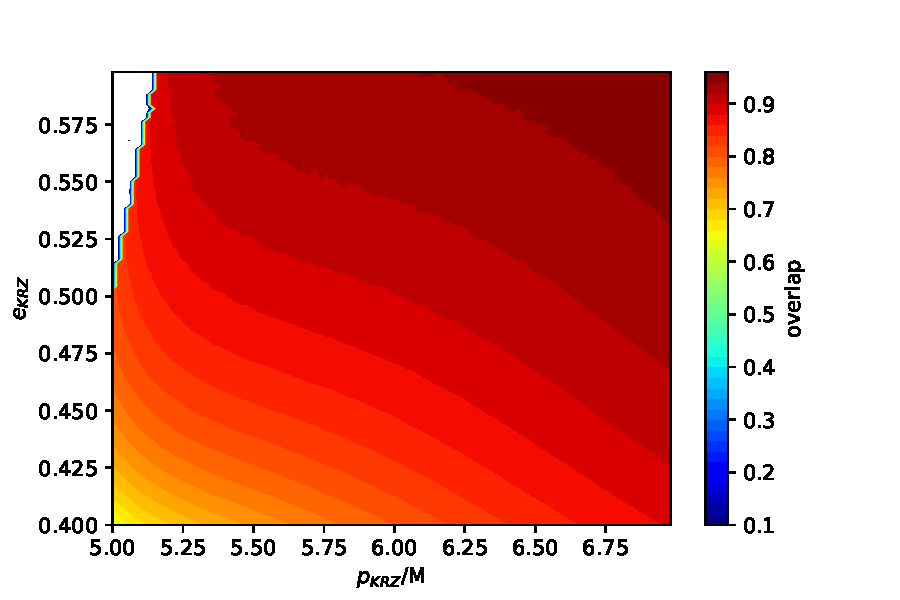
\includegraphics[width=10cm]{ep_best_dist.pdf}
	
	\caption{distribution of overlap between waveform of ($\delta_1,\, a,\, M,\, e,\, p$) = (0.2, 0.5, $2 \times 10^5 $ , $e_{\rm{KRZ}}$, $p_{\rm{KRZ}}$) and Kerr waveform with identical $\omega_r$ and $\omega_\phi$ by varying $e_{\rm{Kerr}},\, p_{\rm{Kerr}}$. The grid size is 100*100. The blank region is unstable orbits.}
	\label{epdist}
\end{figure}	

	\begin{figure}[!ht]
	\centering
	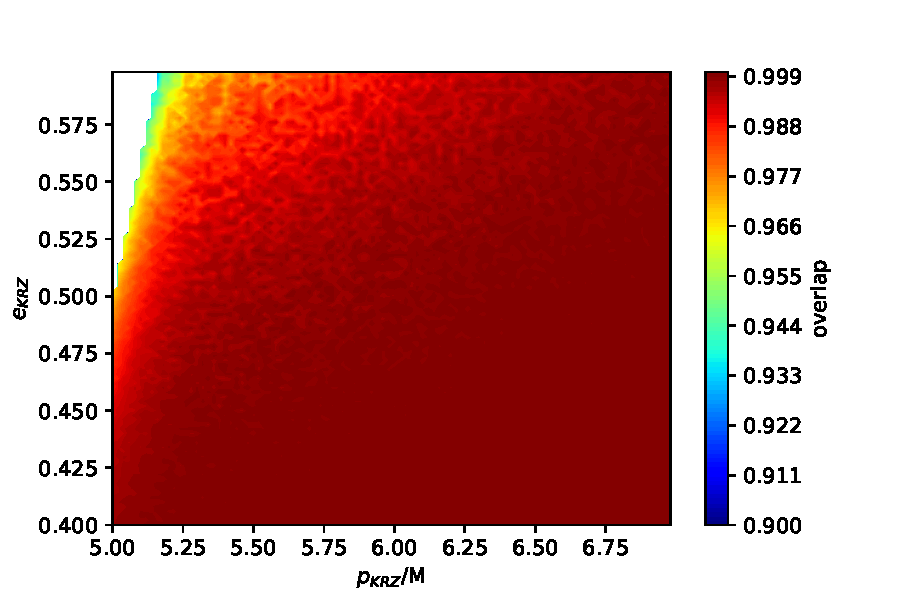
\includegraphics[width=10cm]{FF_am.pdf}
	
	\caption{distribution of overlap between waveform of ($\delta_1,\, a,\, M,\, e,\, p$) = (0.2, 0.5, $2 \times 10^5 $ , $e_{\rm{KRZ}}$, $p_{\rm{KRZ}}$) and Kerr waveform with identical $\omega^{(t)}$ by varying $M_{\rm{Kerr}},\, a_{\rm{Kerr}}$. The grid size is 100*100. The blank region is unstable orbits.}
	\label{amdist}
\end{figure}	

Since metric deformation is more evident near BH horizon, we look at waveforms generated by trajectories close to innermost bound orbit. We compare waveforms of ($\delta_1,\, a,\, M,\, e,\, p$) = (0.2, 0.5, $2 \times 10^5 $ , $e$, $p$) and Kerr orbits varying $(e,p)$ or $(M,a)$ in a 50*50 grid of $(e,p)$. Contour plots of waveform overlap when varying $(e,p)$ and $(M,a)$ are shown in Fig. \ref{epdist} and \ref{amdist}. The confusion problem exists when varying $(M,a)$ for most region we considered. 

\begin{figure}[!ht]
	\centering
	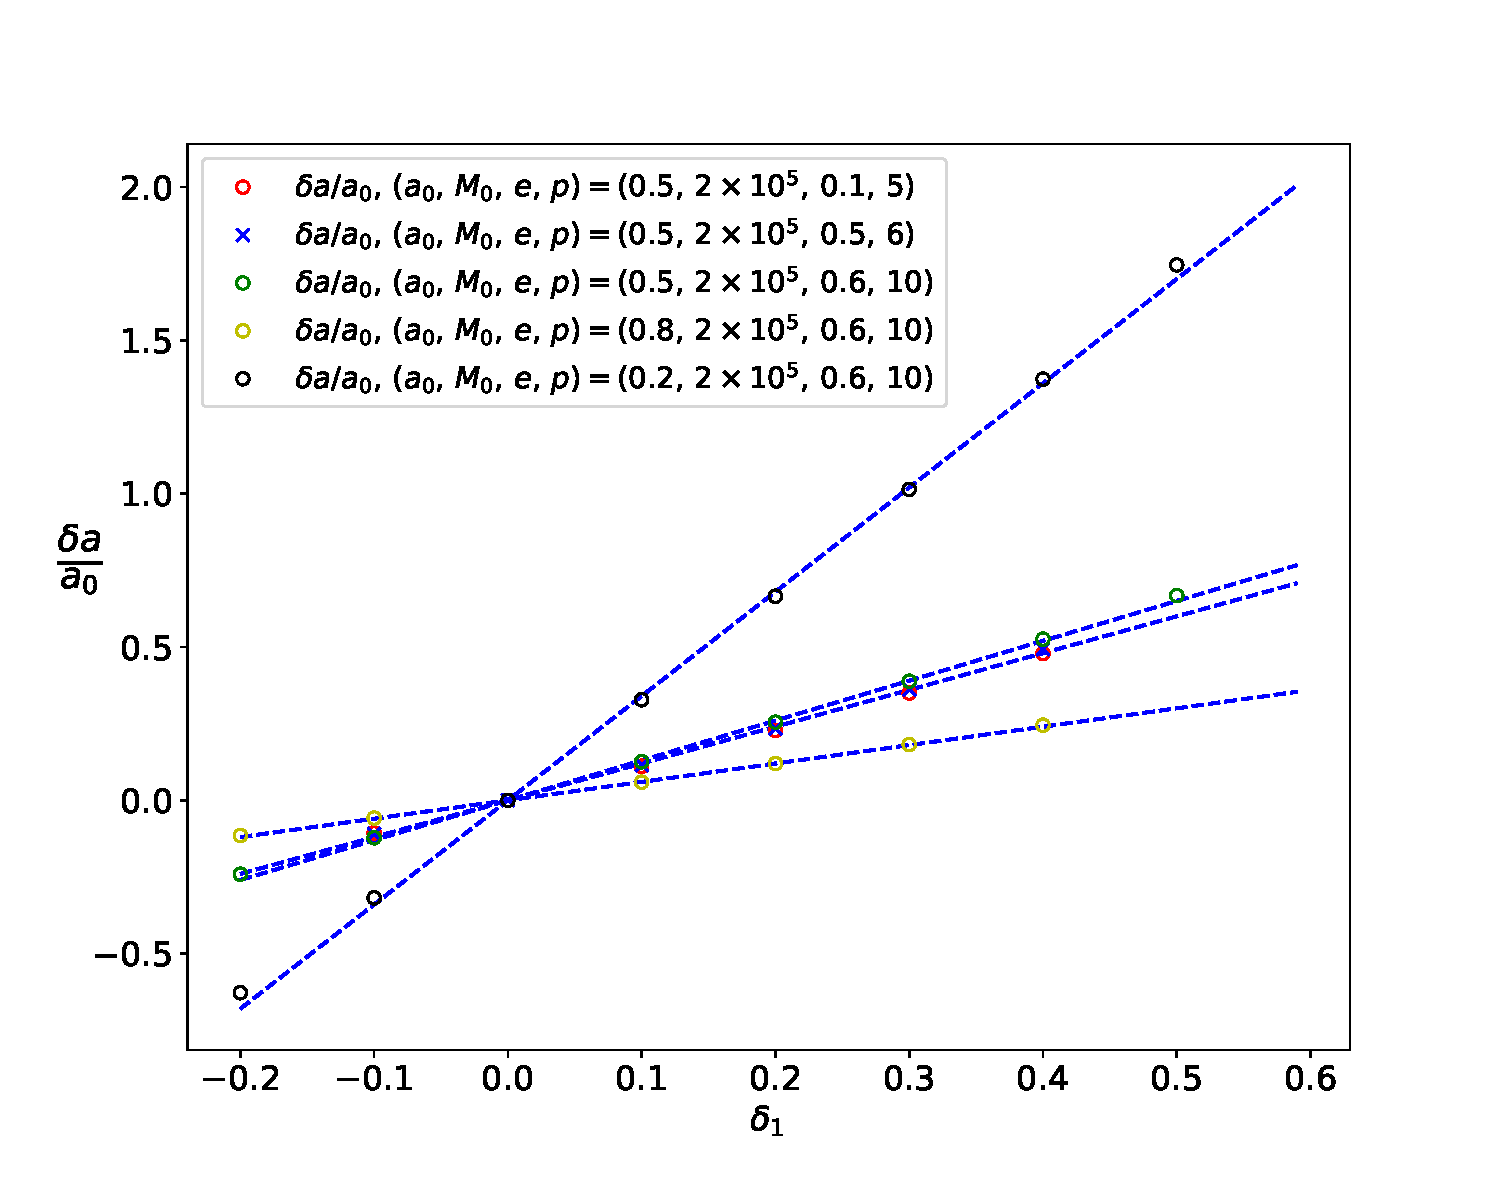
\includegraphics[width=7cm]{d1_spin_linear.pdf}
	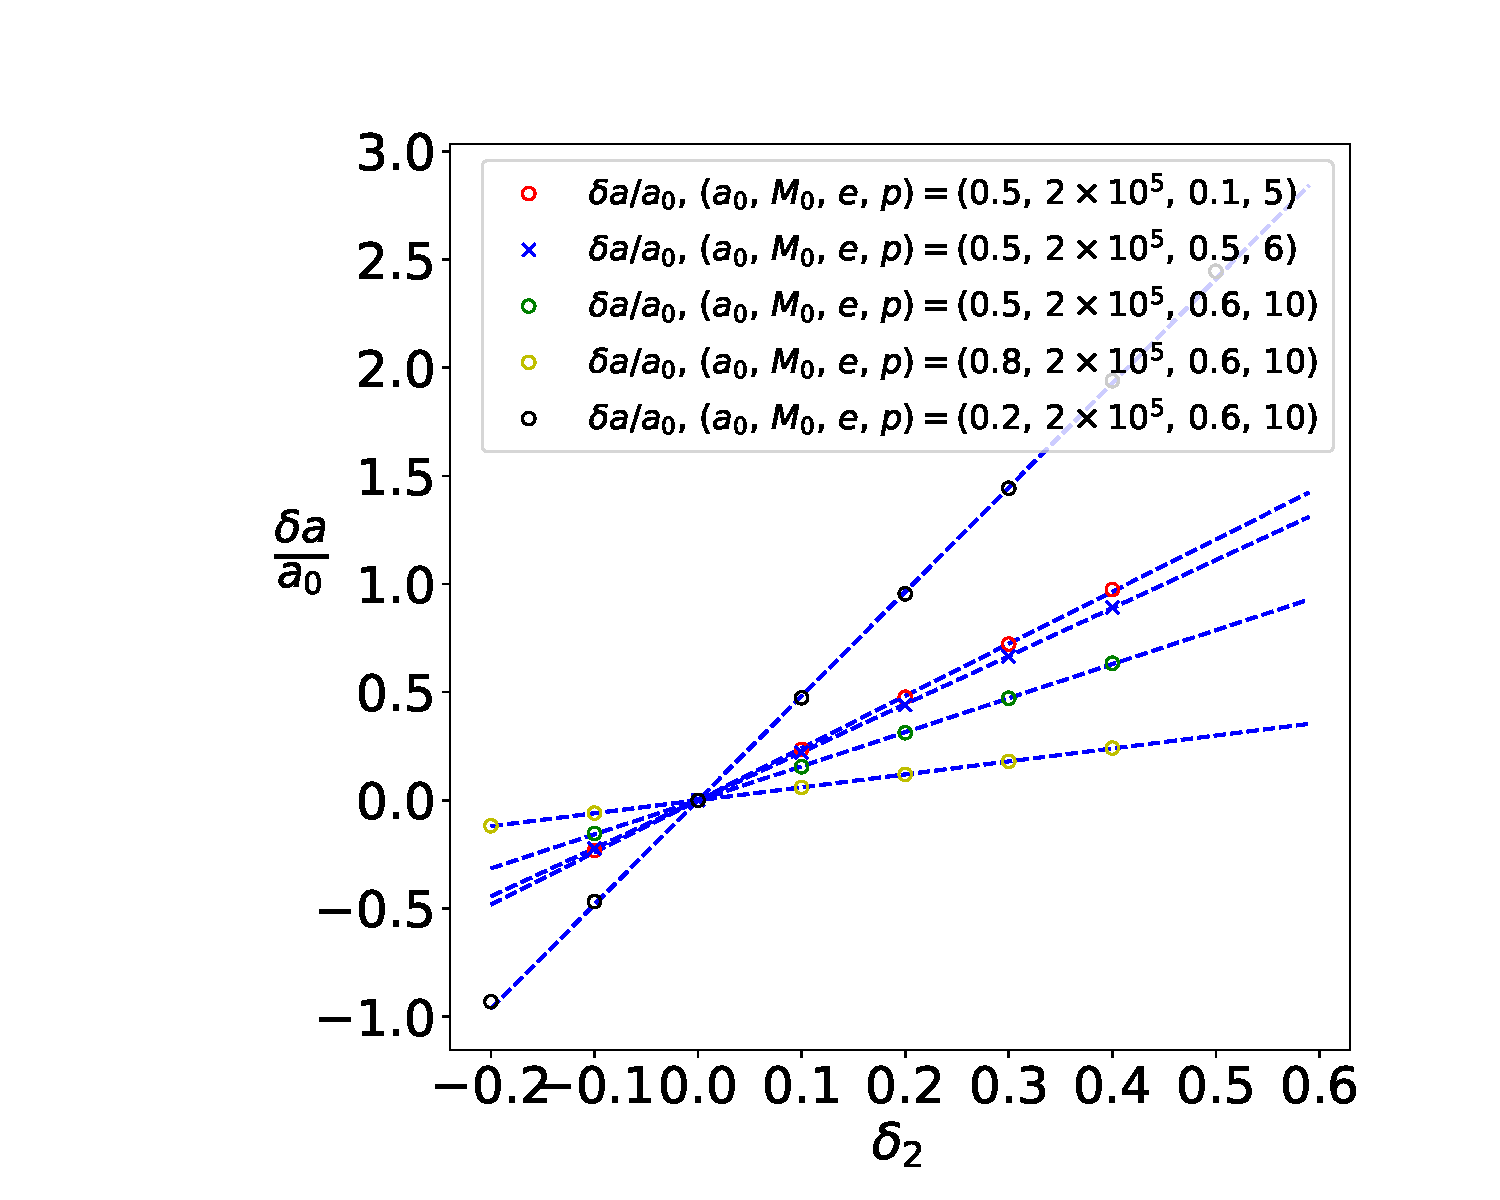
\includegraphics[width=7cm]{d2_spin_linear.pdf}
	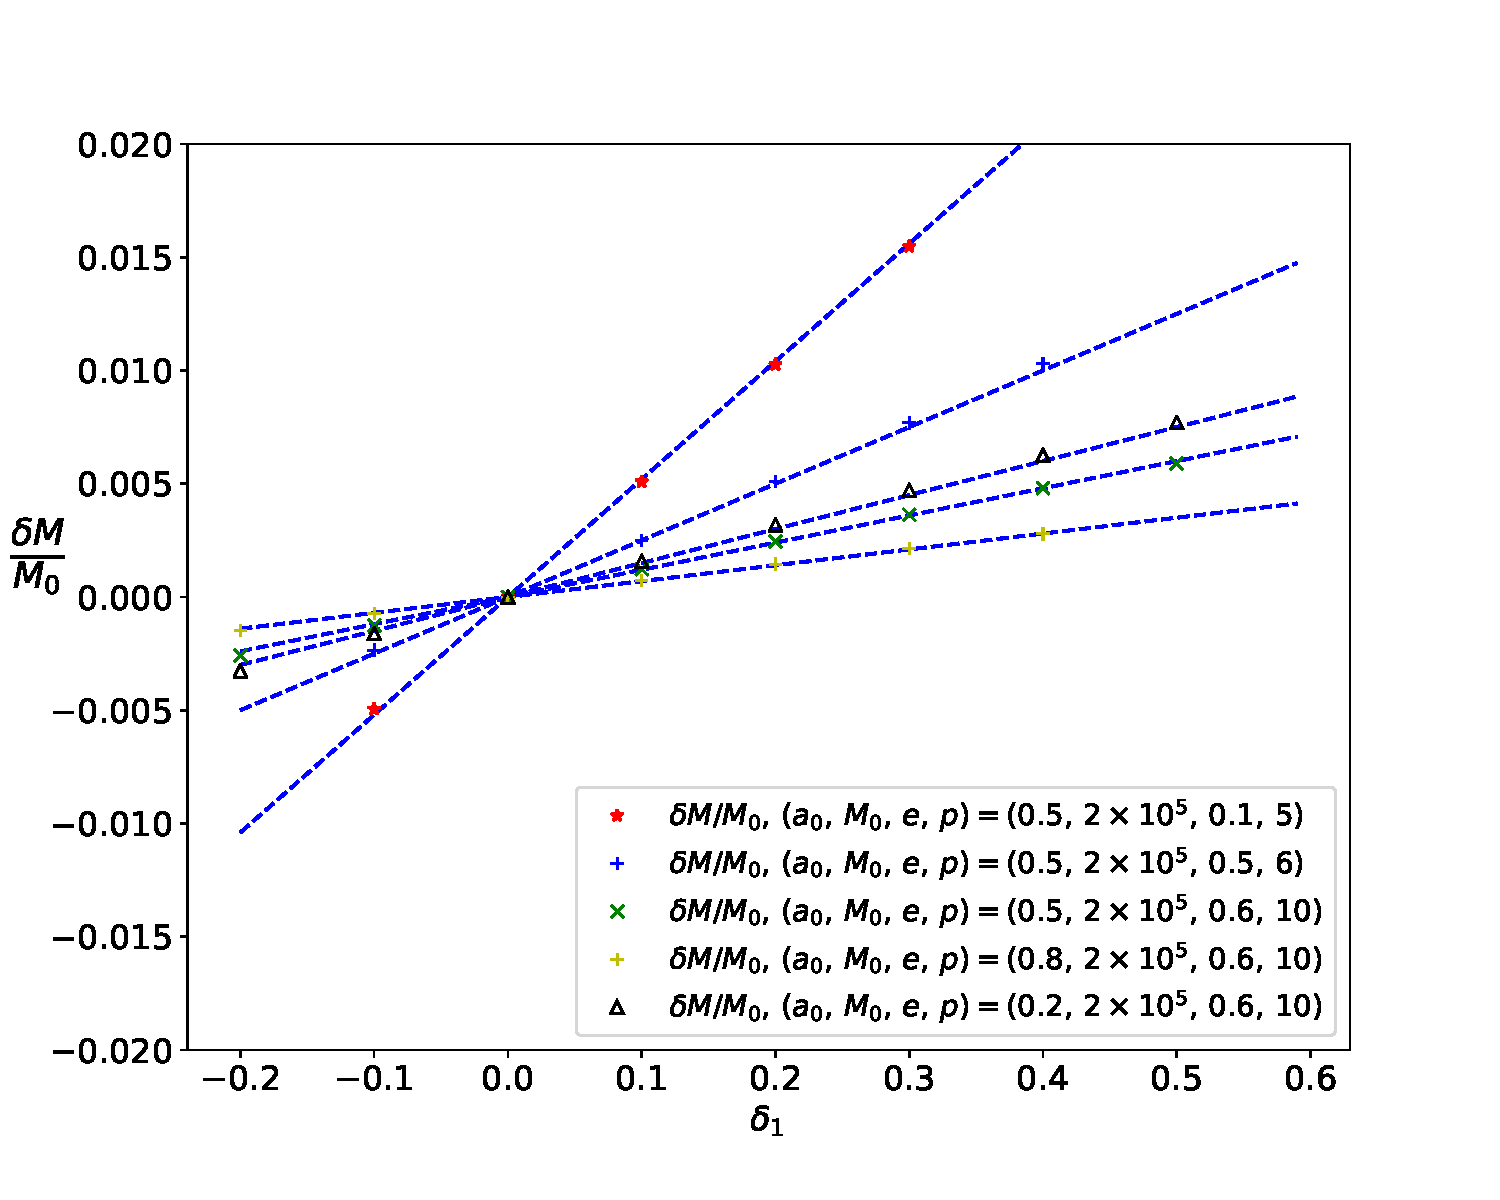
\includegraphics[width=7cm]{d1_M.pdf}
	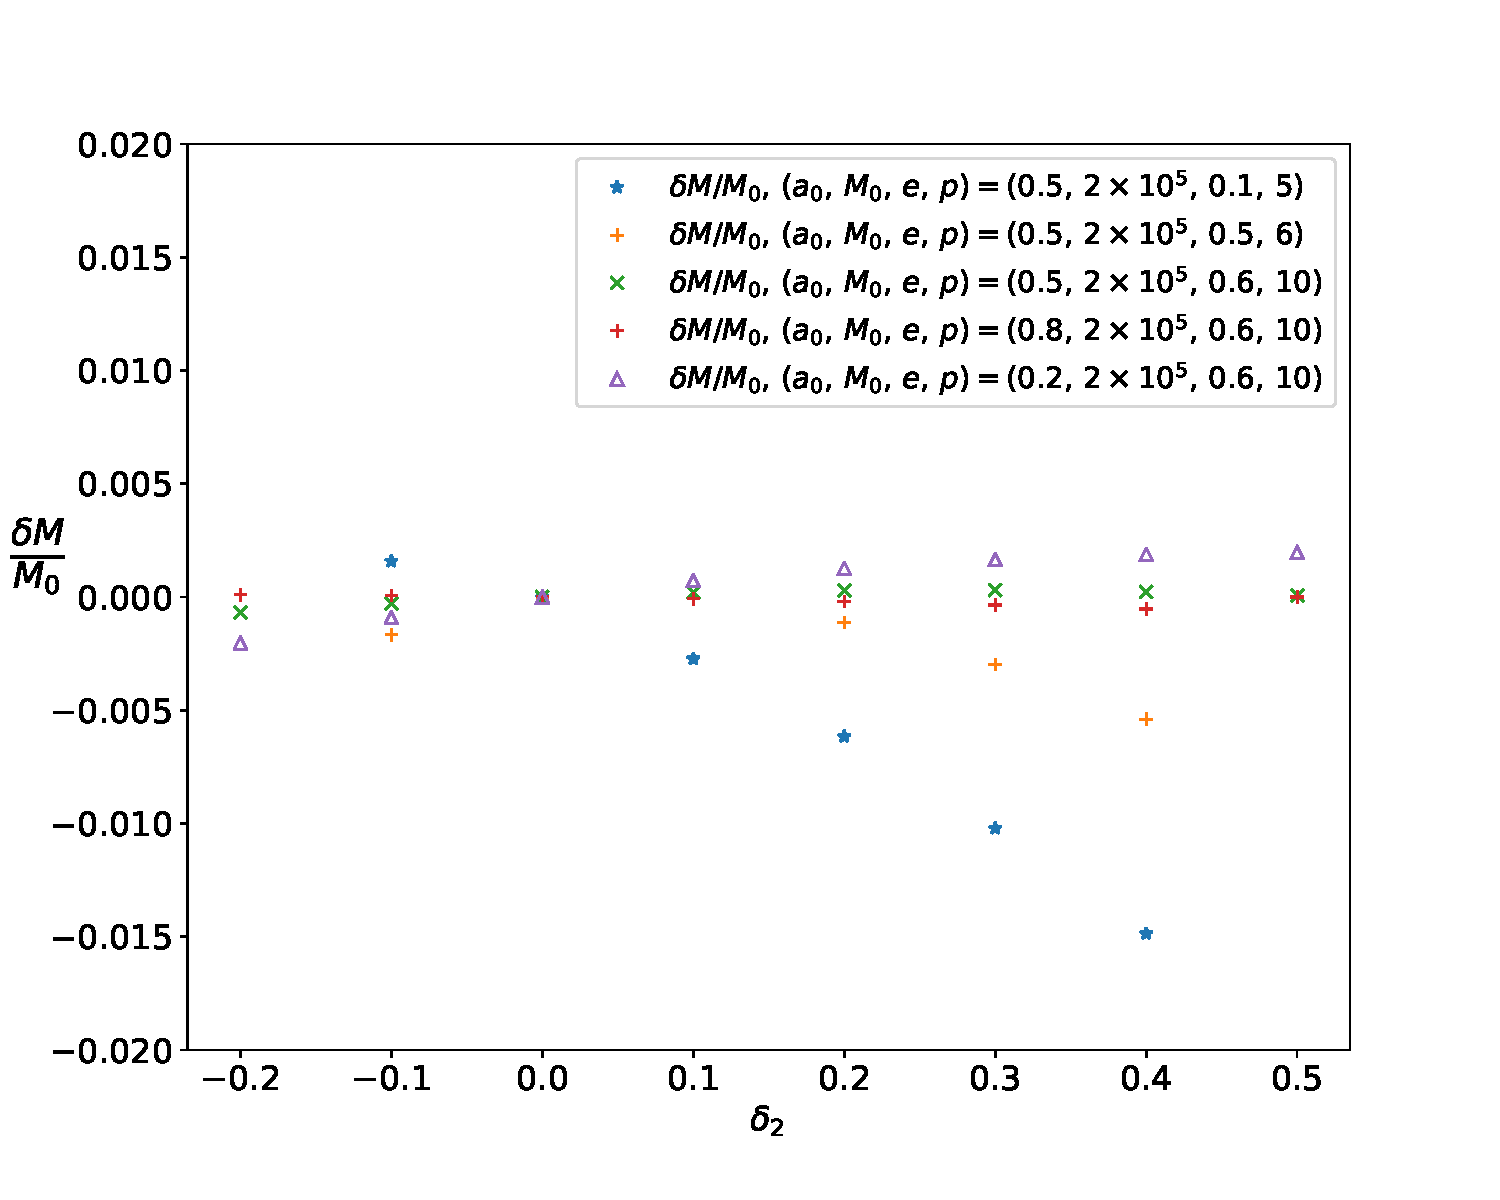
\includegraphics[width=7cm]{d2_M.pdf}
	\caption{relation between relative varied spin/Mass when equating orbital frequency, i.e. orbit of $(\delta_i, a_0, M_0,e,p)$ and $(0,a_0+\delta a, M_0+\delta M,e,p)$ have same orbital frequencies and here shows $\frac{\delta a}{a_0}$-$\delta_i$ or $\frac{\delta M}{M_0}$-$\delta_i$ relations. top left panel: relations of $\frac{\delta a}{a_0}$ or $\frac{\delta M}{M_0}$ to $\delta_1$, top right panel: relations of $\frac{\delta a}{a_0}$ or $\frac{\delta M}{M_0}$ to $\delta_2$.}
	\label{da_linear}
\end{figure}

\begin{figure}[!ht]
	\centering
	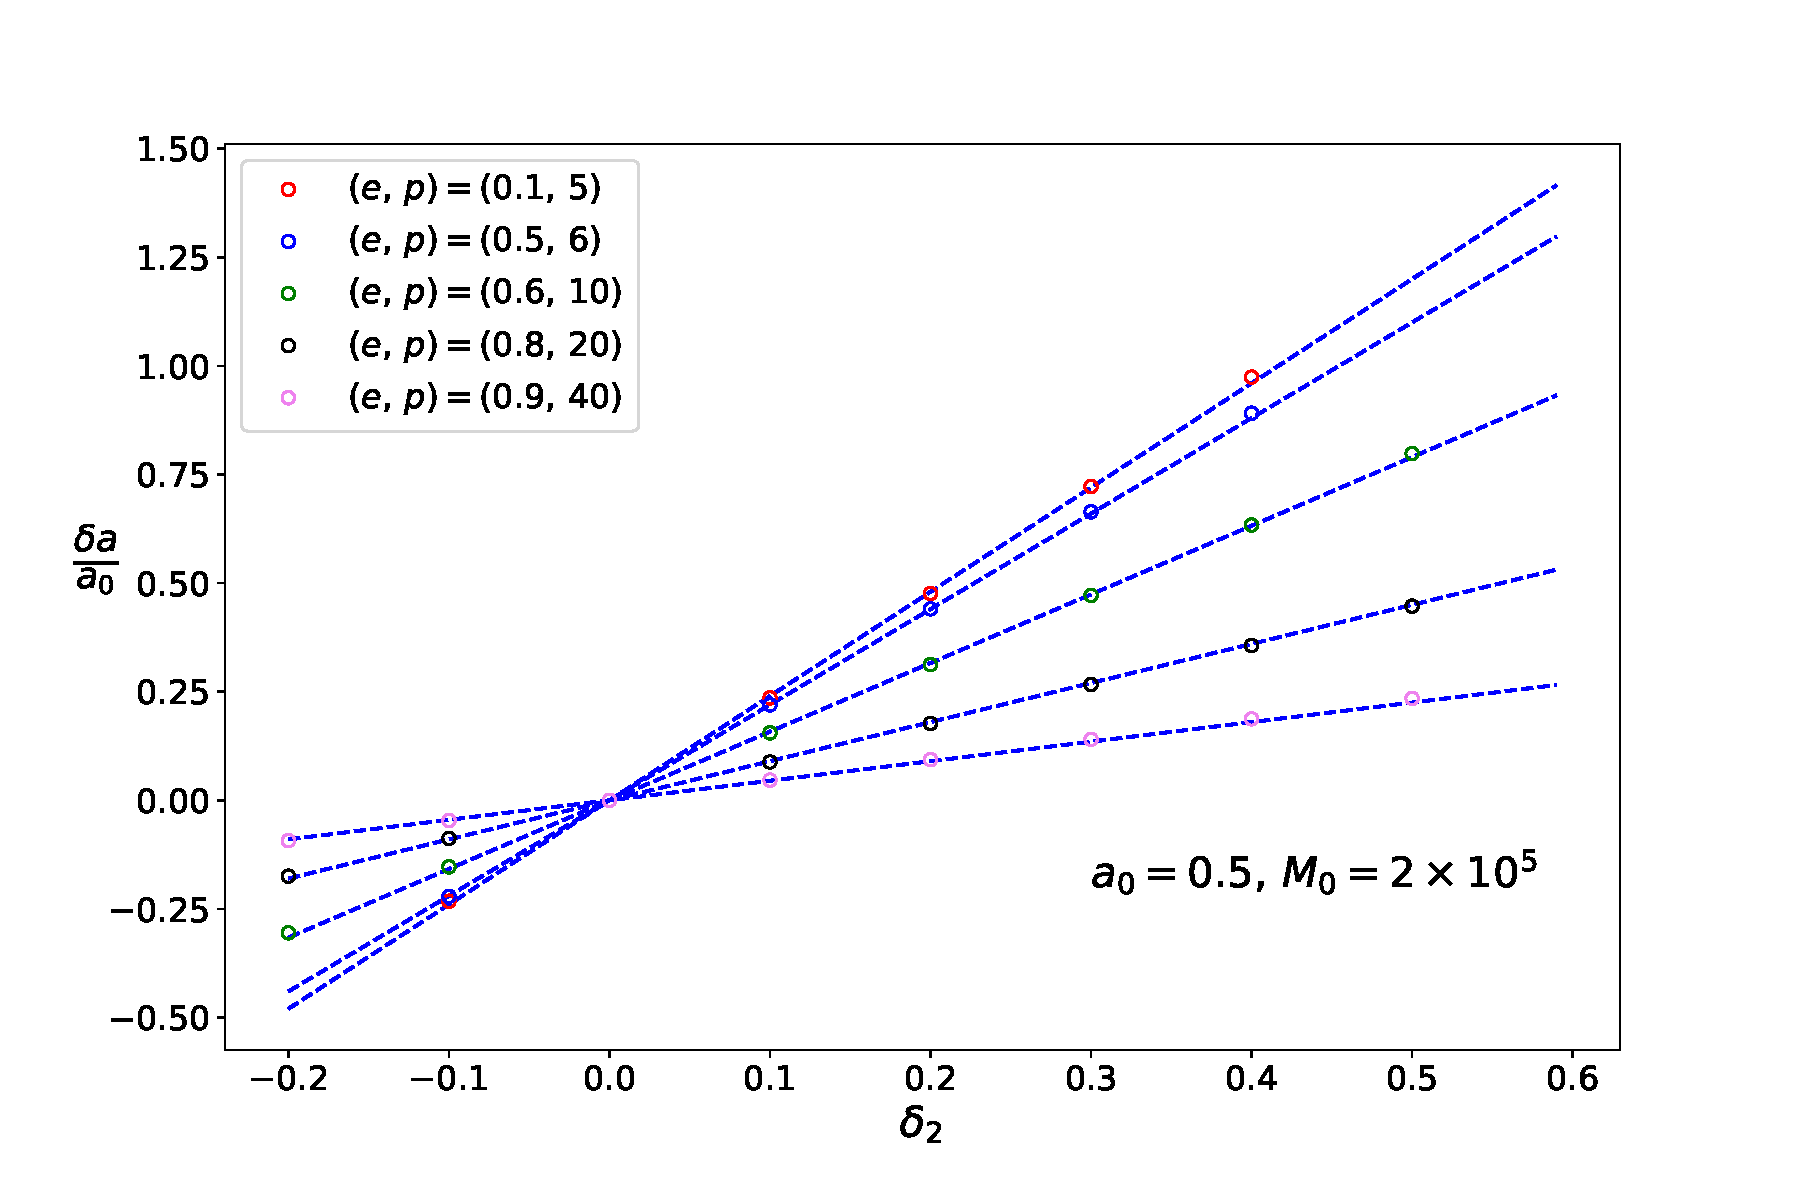
\includegraphics[width=8cm]{d2_deltaspin_ep.pdf}
	
	\caption{Same as Fig. \ref{da_linear}, but only for $\delta a/a_0$-$\delta_2$ relations for different orbits.}
	\label{ep_slope}
\end{figure}

Furthermore, the confusion problem exists for a large range of deformation parameter. When changing the deformation parameter, we found a almost linear relation between $\delta_i$ and varied BH spin/mass, $a_{\rm{Kerr}}$ and $M_{\rm{Kerr}}$, as shown in Fig. \ref{da_linear}. Fig. \ref{ep_slope} shows that slope of this "linear" relation varies greatly for different $(e,\,p)$, so the relation is not a property intrinsic to the metric but dependent on the orbit. The linearity is not a result of small deformation. In fact, as shown in the two figures, the spin varies up to one or two times the spin in KRZ metric. 

\begin{figure}[!ht]
	\centering
	\includegraphics[width=7cm]{2D_bound.pdf}
	\includegraphics[width=7cm]{2D_bound_d2.pdf}
	
	\caption{Upper and lower limit of $\delta_i$, whose waveform can be confused with Kerr waveform, on $delta_i$-$a_{\rm{KRZ}}$ parameter plane, set by equatorial orbit requiring $a_{\rm{Kerr}}<1$ and stable orbit. Other parameters are set to: eccentricity $e=0.5$, semi-latus $p=6.0$ and Balck hole mass $M=2\times10^5$ solar mass. Waveforms in red parameter region, when trying to equate orbital frequencies by varying $(M,a)$, results in $a_{\rm{Kerr}}$ larger than 1. Waveforms in blue region can be confused with Kerr waveform. Orbits in yellow region do not exist. Left panel: for $\delta_1$ and $\delta_2$ set to 0. Right panel: for $\delta_2$ and $\delta_1$ set to 0. }
	\label{d2limit}
\end{figure}

Therefore, for a given orbit parameter $(e,\, p)$, we can regard the introduction of $\delta_i$ as adding the black hole spin and mass proportionally. This sets an limit for the range of deformation parameters within which we can play the trick of varying $(M_{\rm{Kerr}},\, a_{\rm{Kerr}})$. The upper limit is set by requiring $a_{\rm{Kerr}}<1$ and the lower is limited by $a_{\rm{Kerr}}>0$ or stable orbit, e.g. for $(e,\, p)=(0.5,\, 6.0)$, when $a_{\rm{Kerr}}$ is small, the orbit is no longer stable and bounded. Fig. \ref{d2limit} shows the upper and lower bound of deformation parameters with respect to BH spin for orbit with $e=0.5,\, p=6.0$. 

\subsection{Inclined orbit}
\label{p_3d}
Equatorial orbits set some special conditions, i.e. number of orbital frequencies is equal to number of Kerr BH parameters. Therefore, in general we can solve mass and spin by the two frequency requirements set by KRZ orbit, and the resulted geodesics are almost identical. However, astrophysical EMRIs are usually generated by inclined orbits, which have three orbital frequencies. In such cases we usually cannot equate the three frequencies by only varying BH parameters. 

\begin{figure}[!ht]
	\centering
	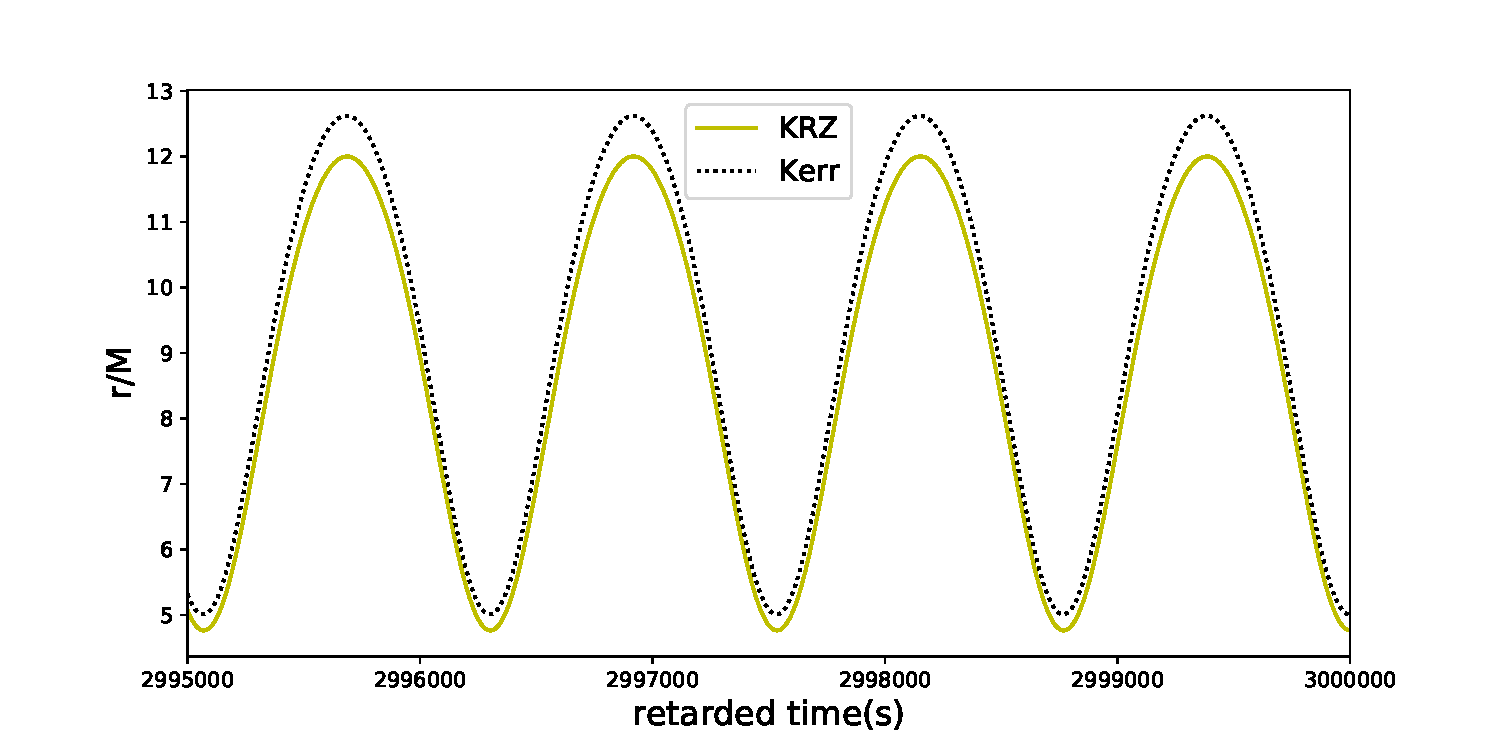
\includegraphics[width=7cm]{r3d.pdf}
	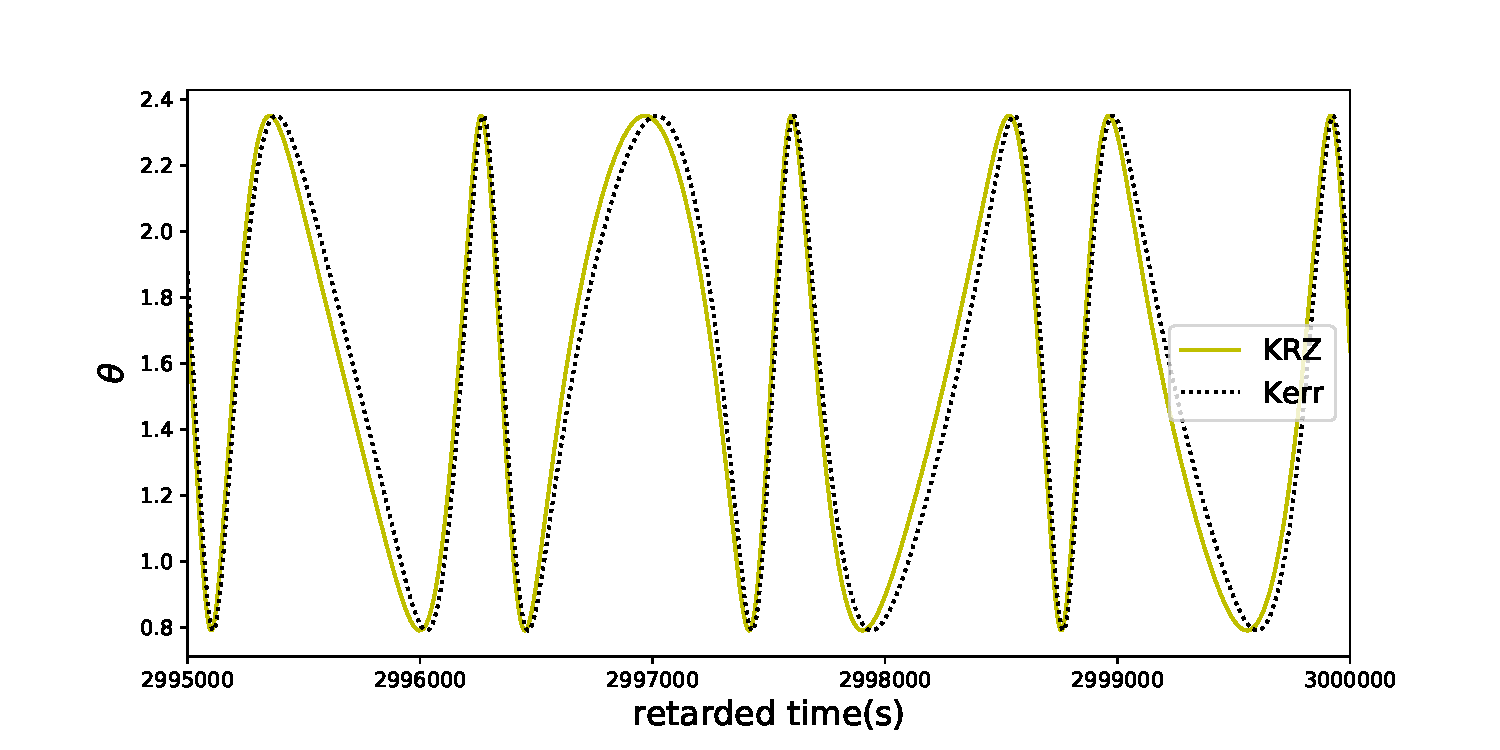
\includegraphics[width=7cm]{th3d.pdf}
	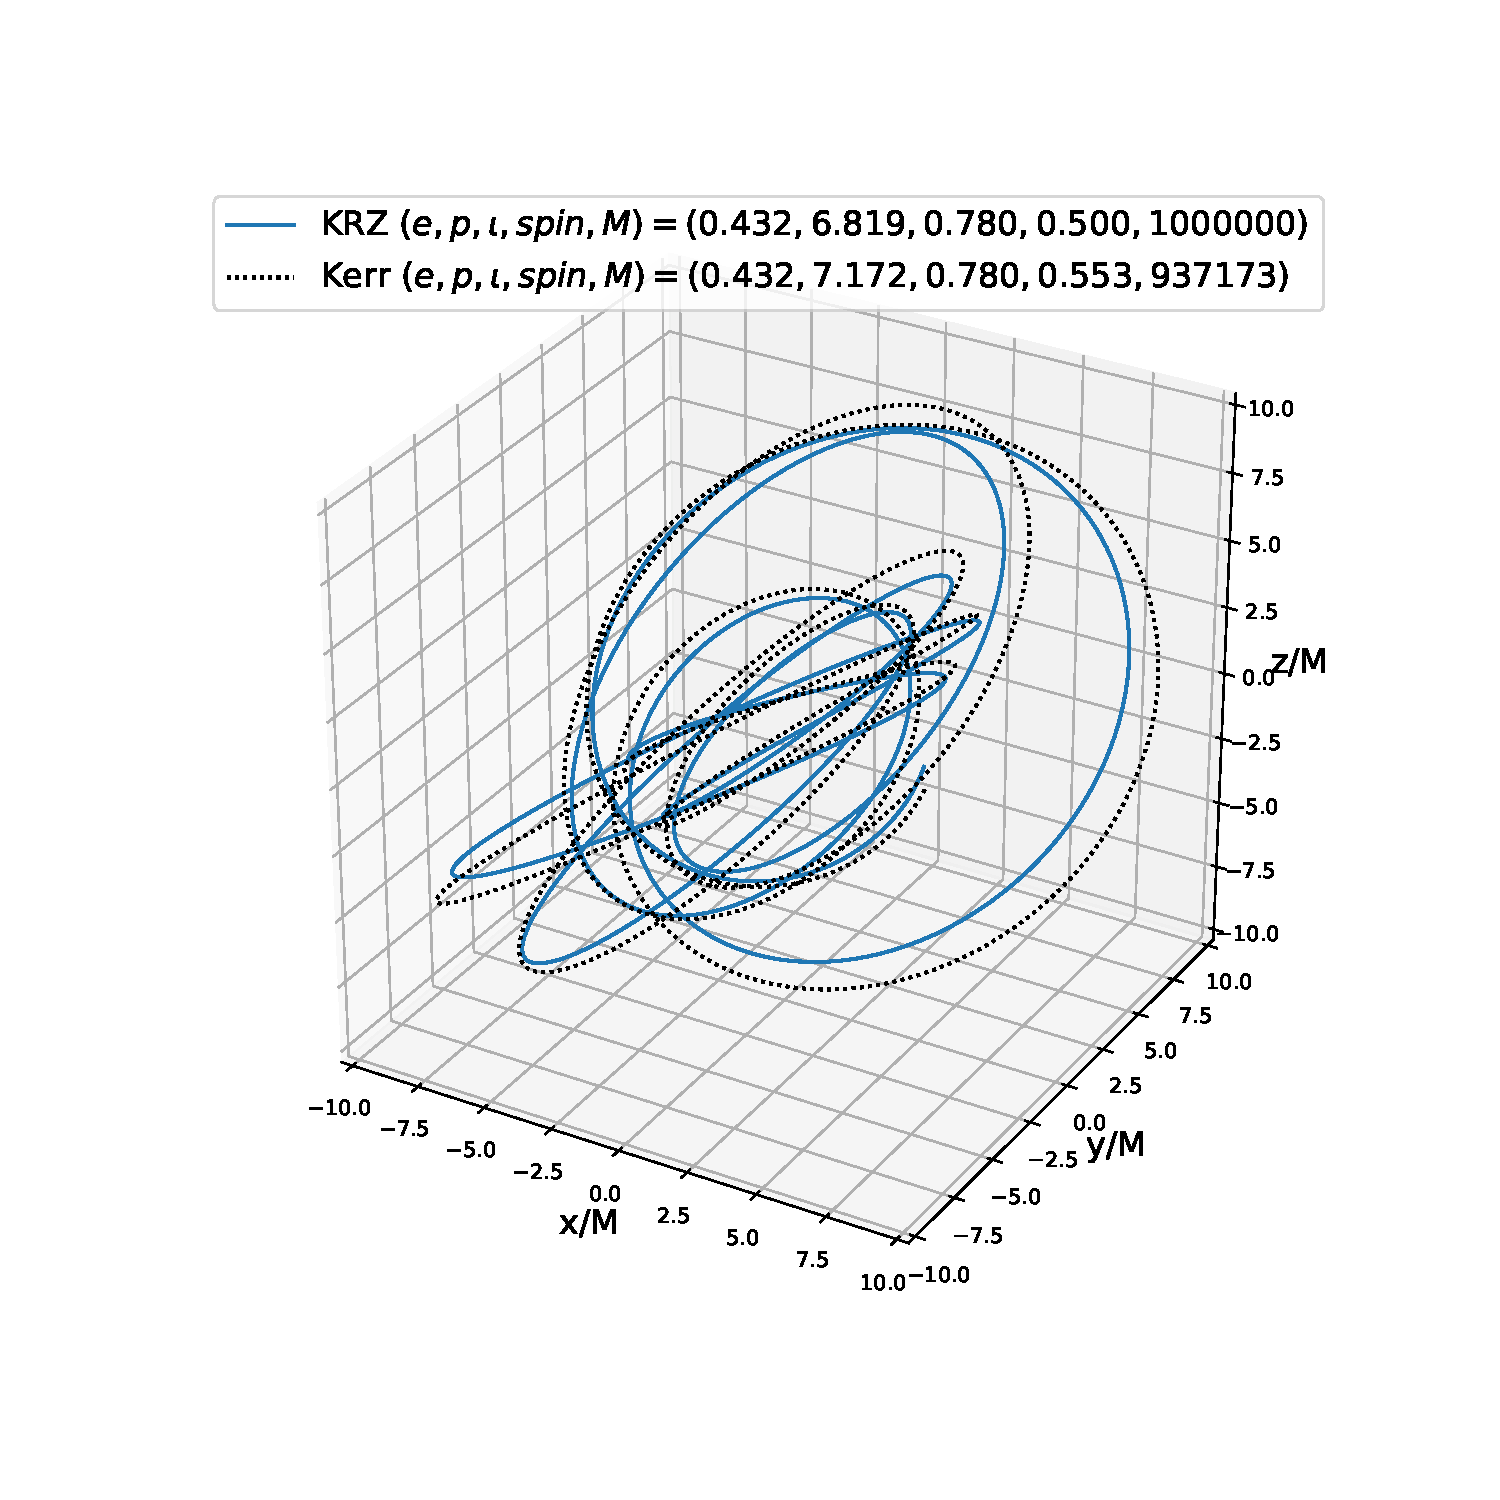
\includegraphics[width=7cm]{trace3d.pdf}
	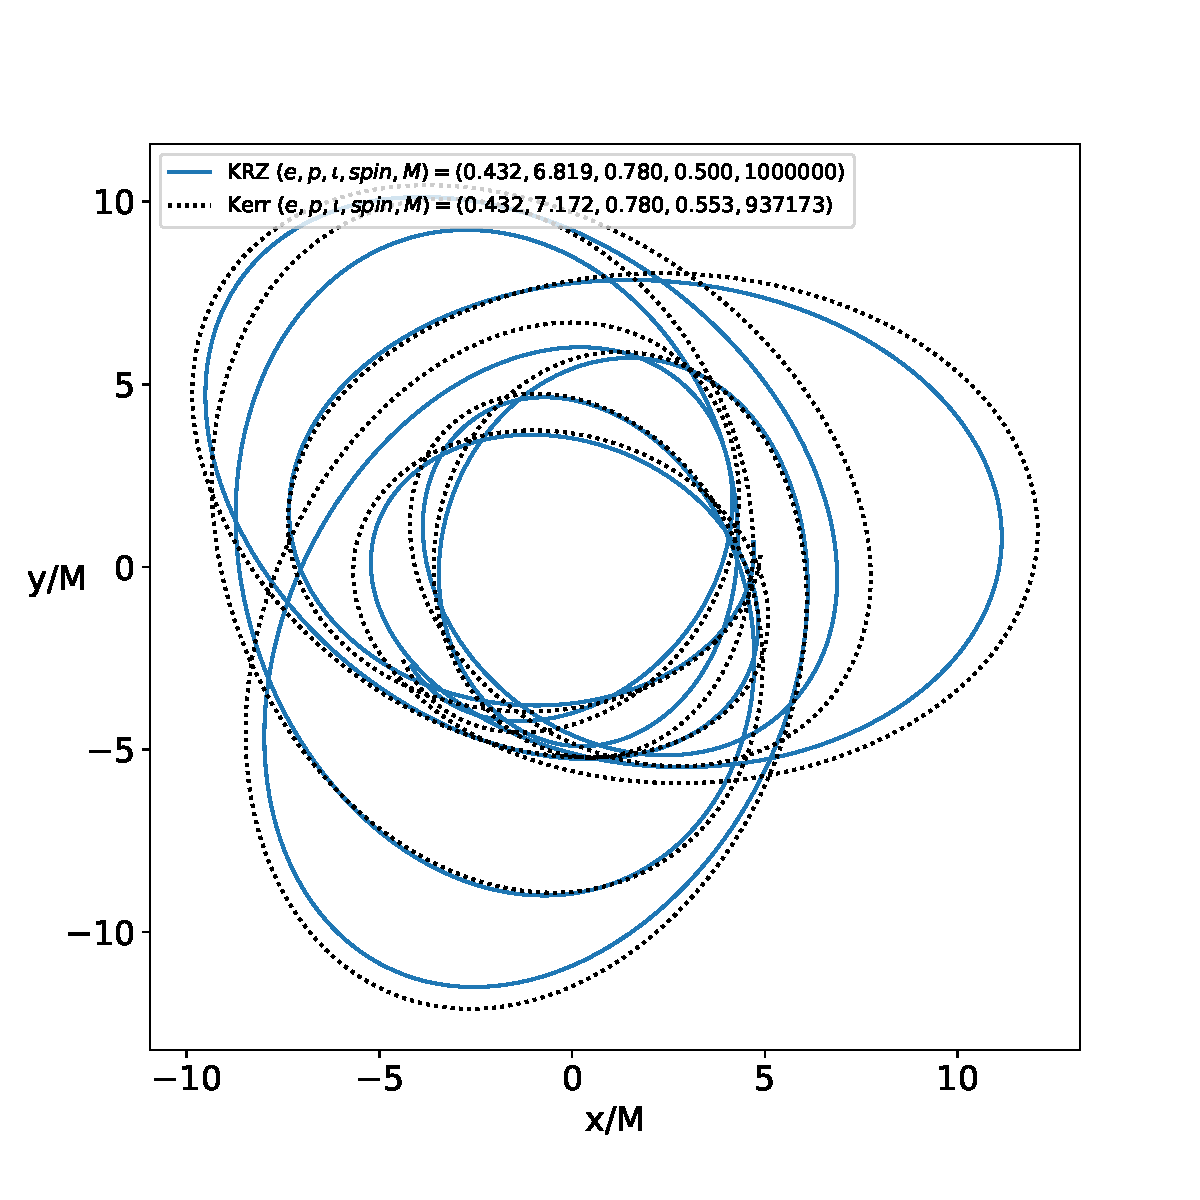
\includegraphics[width=7cm]{tracexy.pdf}
	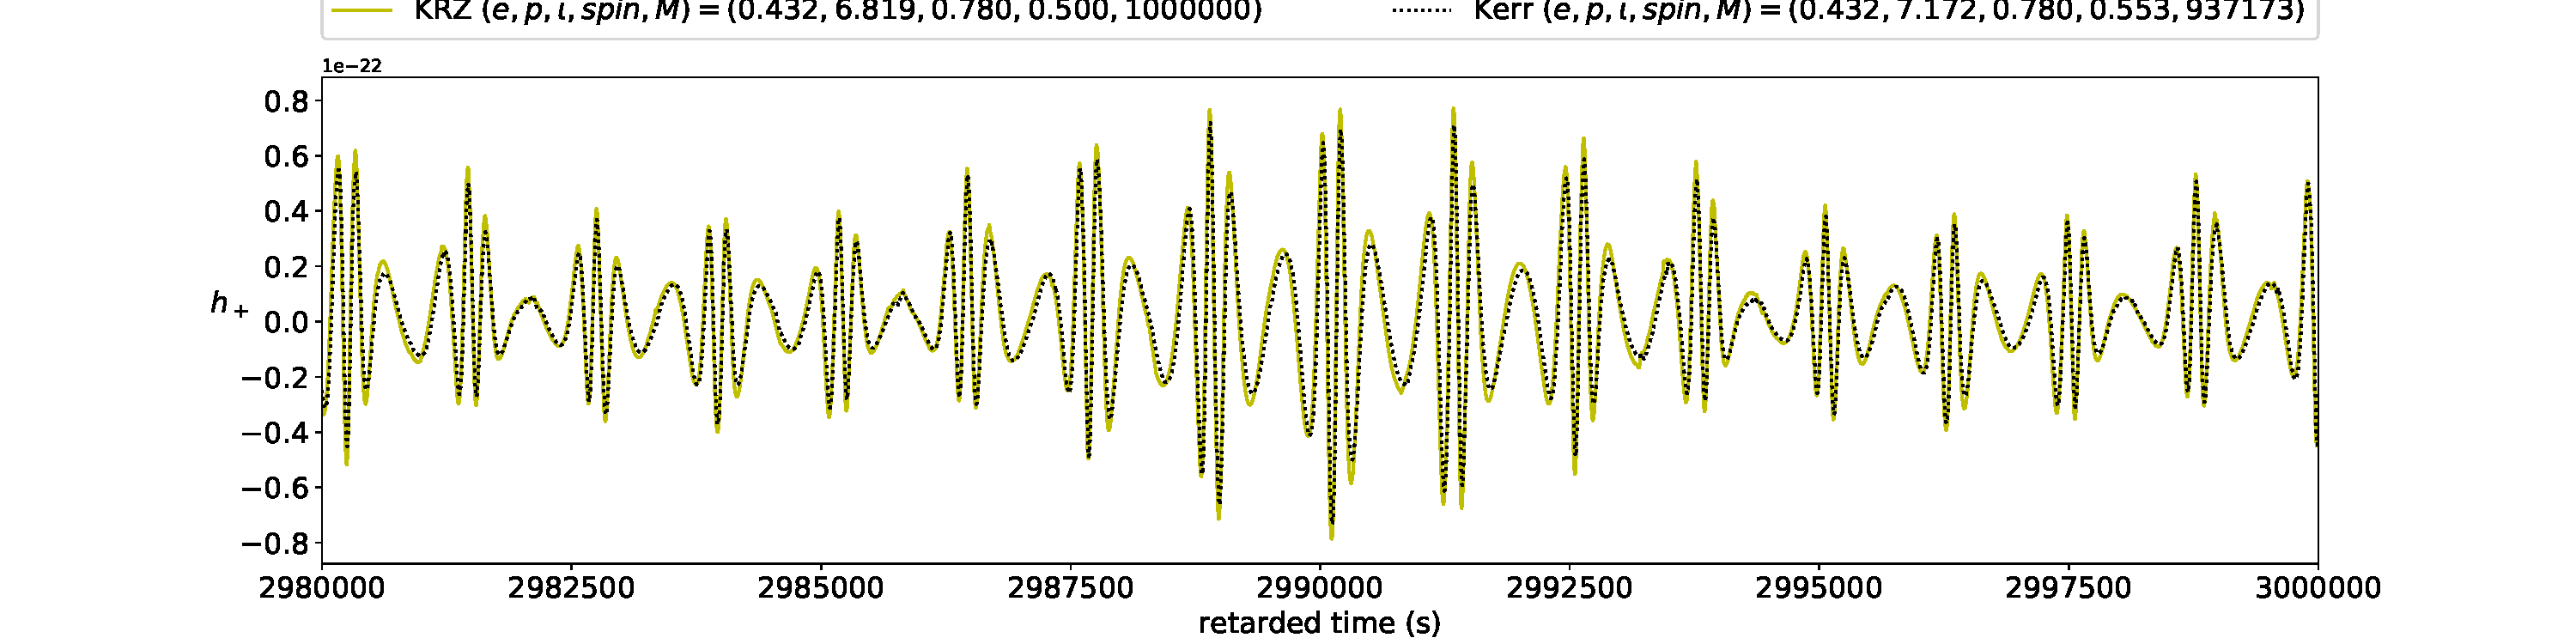
\includegraphics[width=14cm]{wave_d102.pdf}
	
	\caption{Orbits and GW waveforms of a KRZ orbit and a Kerr one with same orbital frequencies. Top left panel: time series of motion in r direction in last 5000s. Top right panel: time series of motion in $\theta$ direction in last 5000s. Middle left panel: trajectories in last 5000s. Middle right panel: projection on xy-plane of the trajectories in last 5000s. Bottom panel: "plus" component of EMRI waveform in last 20000s. The orbit parameters and BH spin/Mass are $(e,p,\iota,spin,M)=(0.432,\, 6.819,\, 0.780,\, 0.5,\, 10^6)$. The deformation parameter of the KRZ orbit is $\delta_1=0.2$.}
	\label{3dtraj}
\end{figure}

However, we found that by varying $(M,\, a,\, p)$ to equate three orbital frequencies, the resulted gravitational waveforms also have an overlap over 0.97, even though the orbits are apparently not identical. Upper and middle panel of Fig. \ref{3dtraj} show the time series of motion in $r,\, \theta $ direction and trajectories in the last 5000s, the total time is $3\times 10^6$s. Motion at $\theta$ direction is almost overlapping with a few distortions. Motion at $r$ direction has the same frequency but different amplitude, basically resulted from varying the semi-latus $p$. However, the gravitational wave signal are almost identical as shown in the bottom panel. 

\begin{figure}[!ht]
	\centering
	\includegraphics[width=8cm]{3D_bound.pdf}
	
	\caption{Same as Fig. \ref{d2limit}, but for inclined orbit and waveform at each point is determined by setting initial $E,Lz$ same as corresponding Kerr orbit, see text for details.}
	\label{3dlimit}
\end{figure}

Similar to equatorial cases, requirements of $a_{\rm{Kerr}}<1$ and stable orbits set bound to the deformation parameters. However, since there's no carter-like constant in KRZ metric, we cannot control orbit parameters $(e,\, p,\, \iota)$. Therefore, we try just to control the initial condition so that the orbit parameter are at least near the desired value, e.g. $(e,\, p,\, \iota) = (0.2,\, 8,\, \pi/4 )$. Technically, given $\delta_i$, $a_{\rm{KRZ}}$ and reference orbit parameter, we calculate the energy $E_{\rm{Kerr}}$ and angular momentum $L_{z -Kerr}$ in Kerr spacetime with spin equal to $a_{\rm{KRZ}}$, then set the initial coordinate as $\theta=\pi/2$, $\phi=0$, t=0 and r at $\frac{p}{1-e}$, set $E,\, L_z$ equal to the Kerr value, which determines velocity in $t$ and $\phi$ direction, set $u^r=0$ and $u^\theta$ is determined by modulus of 4-velocity. The upper and lower bound of deformation parameters determined in this way is shown in Fig. \ref{3dlimit}. $M_{\rm{KRZ}}$ is $10^6$ solar mass and total time is $2\times 10^6$s.


\section{Conclusion and Discussion}
\label{p_fin}

%用了什么方法
LIGO's detection of GW signal has opened up the era of gravitational wave physics. Future LISA task will be able to extend our sight over a broader spectrum in GW signals. One scientific goal of LISA task is to test Kerr metric or No-Hair Theorem in strong field region, but the "confusion problem" is still a burden. In this paper, we consider the general parametrized metric of axisymmetric BHs, namely KRZ metric. With Kludge method for waveform generation, we investigate the confusion between EMRI waveforms under Kerr metric and KRZ non-Kerr metric. We mainly consider deformation parameters $\delta_1$ and $\delta_2$. For both equatorial and inclined orbits, we study the overlap between waveforms of same orbital frequencies.

%结果是什么,意义是什么
The results show that the confusion exist in a large range of parameter space for both equatorial and inclined orbits, within the small and medium deviation ($\delta_i<1$) region. However, for high spin and deviation $\delta_i>0$, it is still possible to discern the back ground metric by physical restriction, $a_{\rm{Kerr}}<1$. In equatorial cases, for a given orbital parameters $(e,p)$ the increase of $\delta_i$ is almost equivalent to proportional adding BH spin in Kerr metric, as far as waveforms are considered. Therefore, when matching EMRI waveform to test the background metric, care must be taken to check the ``confusion problem''. 

%展望
But the ``confusion problem'' we have considered does not rule out the possibility of discerning BH metric with LISA detection. By a longer period of observation, where radiation reaction plays a more significant role, we could possibly observe the difference in orbit evolution by studying EMRI signal. For EMRIs with confusion problem from inclined orbits with same orbital frequencies, the semi-latus $p$ is different for Kerr and non-Kerr cases. Therefore the radiation flux of the GW is different and this can lead to different orbital evolution over longer time scale. Also, the confusion may be a result of approximation of waveform generation methods, which ignore higher order contributions to GW signals. In the future, we will extend our analysis to waveforms generated by more accurate methods and add radiation reaction over longer time scales. 

%用别的方式确定spin/mass, multimessenger: GW+ Xray+ neutrino
Another way out is multi-messenger measurements. \cite{measureBHspin}


\bibliography{citation}
\bibliographystyle{plain}
\end{document}